\section{System design}
In this chapter, the design of the system is explained.
The focus of section 3.1 will be an overview of the first approach implemented, the ring topology. Here, a detailed analysis this architecture and its trade-offs is presented. Similarly, in section 3.2 there is an analysis of the second approach implemented with full connectivity. Lastly, in section 3.3 we discuss the additional features implemented in the system. \\\\
All the components of the system have been written using Java 8. In order to communicate across the different nodes, the Java RMI library is used, which
allows methods on different machines to be invoked as methods
of native objects with very little alteration.
For asynchronous computing the LinkedIn ParSeq library [1] was used.
It provides a \textit{Task} abstraction comparable to Java's
unwieldy \textit{Future} implementation.
This abstraction is more similar to objects and methods than the threading
alternative, which is closer to the hardware implementation.
Thus, it makes it easier to reason about the system in terms of tasks and objects than threads and interruptions.

\subsection{Ring topology}

The proposed architecture, depicted in figure 1, consists on a logical ring of GSs and evenly divided groups of RMs.
Each group of RMs is primarily connected to one GS (blue lines) and the next GS in the ring as backup (red lines). Apart from that, every GS is connected to the next and previous GS of the logical ring (black lines). Be connected means to send periodically heartbeats to check if the components are online. 
\\ 
\begin{figure}[H]
\centering
	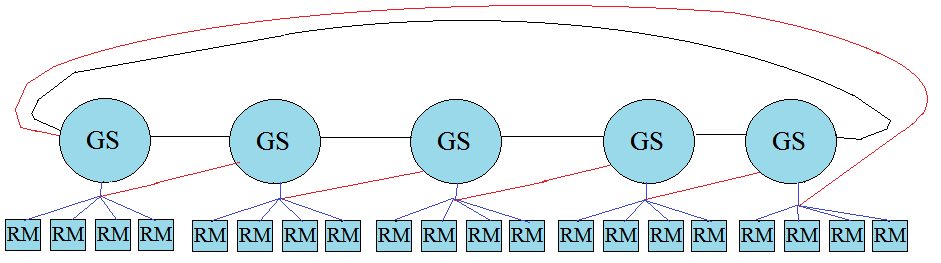
\includegraphics[scale=0.61]{ring.png}
	\caption{Ring topology}
\end{figure}

\subsubsection{Bootstrap}
As in most of distributed computing systems [2], this topology has the bootstrap problem. How to initiate the system? Since the topology is fixed, the components need to know previously with who they are going to be connected with which causes synchronization issues.

\subsubsection{Replication}
When a job request arrives to a cluster controlled by a RM this will check whether it can accept the job or not. If there are resources available, the RM will send a monitoring request to its main GS, this will translate a backup request to the backup GS and return the confirmation to the RM. After that, it will begin the execution of the job in one of its nodes. This replication strategy guarantees that if a RM suspends its activity, the jobs can be rescheduled in another cluster and that in case of failure of one GS or GS/RM at the same time, the remaining GS will be able to reallocate the workload of the failed cluster in another one.

\subsubsection{Fault recovery}
Failures of RM are discovered by the main GS, when this happens the GS will inform the backup GS to stop monitoring the previous RM. After that, it will reallocate the jobs in a new cluster, prior contacting the main GS & backup of that cluster. Once the RM receives the workload from the GS it will schedule and execute it as normal job requests.
On the other hand, when the backup GS detects a failure of the main GS, it will self promote to become the main GS of the cluster under the control of the failed GS. Additionally, the RM will connect to the previous GS on the ring next to the failed one as backup GS.
\\\\
This strategy of fault recovery may seem robust, however, it is likely to trigger a failure of the whole system due to the domino effect. The reason behind it is that all the workload monitored by the failed GS is now supported by the backup. If the latter has already a big amount of jobs under its supervision, it will probably fail, as well as triggering a domino failure. This scenario is also possible in the case of a RM failure. The GS monitoring the new selected cluster will assume all the incoming workload. Moreover, given that when a node crashes all its connections are re-established it is hard to implement the "coming back to life" mechanism.

\subsubsection{Scalability}
This topology scales well as it does not present a message overload. Adding a new GS will just imply connecting the new component to another two GSs and two RMs (one for main monitoring and one for backup). Similarly, including a new RM will just need two new connection to the main and backup GS respectively.

\subsubsection{Load balance}
To maintain a balance among the different clusters, the system will load balance, which means transferring jobs from more loaded clusters to the less ones. However, given the ring topology where a GS only sends message to the two next nodes, message forwarding is required so that all the GSs are aware of the load of all the clusters. This forwarding mechanism is complex and inefficient as introduces latency and new synchronization issues among the nodes.

\subsection{Full connected topology}
Given the issues and complexities of the ring topology described above, we chose to implement a second approach described in the remaining of this subsection. The main characteristic of this topology is that every component sends periodically heartbeats to the rest of the system. A diagram of the topology is depicted in figure 2.

\subsubsection{Bootstrap}
Initializing the system is easier than with the first approach. All the nodes have a list of URLs of the whole system, once started they begin to ping periodically the rest of the nodes. In this way it is possible to maintain a distributed consistent status as every node knows the status of the rest.

\begin{figure}
\centering
	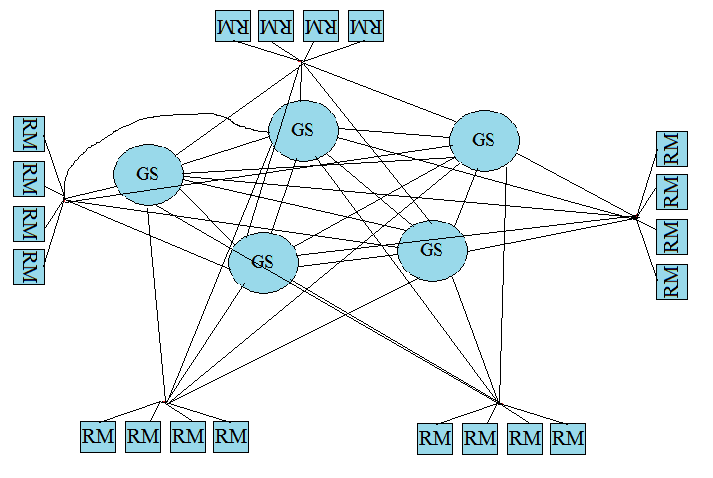
\includegraphics[scale=0.61]{full.png}
	\caption{Full connected topology}
\end{figure}

\subsubsection{Replication}

The replication process is somewhat similar to the ring topology. When a job requests arrives the RM requests for monitoring and the GS selects a proper backup for the workload. However, in this case the main GS and the backup GS are selected following a weighed random fashion. With this strategy we try to avoid overloading a certain grid scheduler.

\subsubsection{Fault recovery}

Failure detection is also similar to the case of ring topology. However, because the monitoring and backup selection is made randomly it is unlikely to trigger a domino failure, making the system more robust. Also, when a crashed node goes back online it will simply notify the rest of the system so it can be selected again for monitoring (in the case of a GS) or contact with grid schedulers for monitoring and backup (in the case of a RM). 

\subsubsection{Scalability}
Regarding the scalability, clearly this topology does not scale well as it scales with $O(|GS|\cdot |GS|-1 + |RM|\cdot |GS|) = O(n^2)$. Where $|GS|$ and $|RM|$ denotes the number of GSs and RMs respectively. The first term $|GS|\cdot |GS|-1$ is the number of heartbeats among the GS, whereas the second term $|RM|\cdot |GS|$ indicates the number of messages between RM and GS. This scalability factor clearly is not good at all, however we have to take into account that the size of the heartbeat is extremely small, it just contains the load of the cluster(s), thus the total overload is not that high.

\subsection{Additional features}

As explained above, the system designed is able to tolerate failures in at most two nodes at the same time. Actually, it can tolerate multiple combinations of failures in GS/RM nodes as long as there are sufficient nodes to support the workload. Going beyond what it was previously said, the system has the ability to deal simultaneously with diverse users since job requests include a user identifier. The different workloads are treated evenly thus, in this way the system offers a best effort service. The fairness of the system will be analyzed in the following section of experiments.